\chapter{Umsetzung} %Beide

\section{Umsetzung der Anwendung} %Benedikt

\section{Umsetzung des künstlichen neuronalen Netzes} %Sebastian

beschreibung folgende 3 abschnitte sukzessive
normalisierungsfunktion
beispieldatensatz (training / test)
verteilung(training/test)
menge(training/test)
Anzahl Durchläuge: 100k
Lernrate 0.5


\section{Optimierung des künstlichen neuronalen Netzes}
\label{section:Optimierung des künstlischen neuronalen Netzes}
\subsection{Optimierung der Topologie} %Sebastian
In der Literatur wird dabei oft auf die folgende Gleichung zur Ermittlung der optimalen  Menge an Neuronen der versteckten Schicht angegeben:

\begin{equation}\formelentry{Optimale Anzahl Neuronen in der versteckten Schicht}
  N_h = \frac{N_d}{10*(N_i+N_o)}
\end{equation}


\begin{figure}[htbp]
\centering
		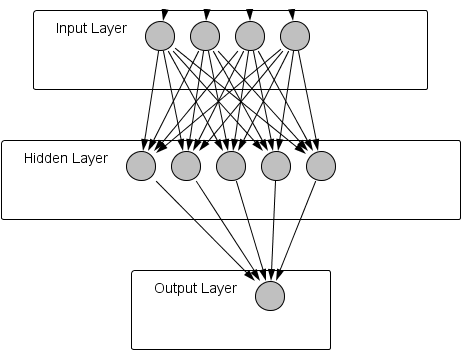
\includegraphics[width=0.75\textwidth]{4-5-1.PNG}
	\caption{KNN nach 4-05-1 Muster}
	\label{fig:KNN nach 4-05-1 Muster}
\end{figure}


\begin{figure}[H]
\centering
		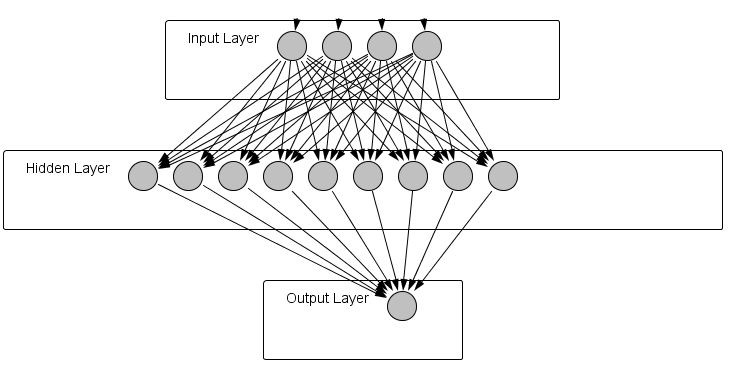
\includegraphics[width=0.75\textwidth]{4-9-1.PNG}
	\caption{KNN nach 4-09-1 Muster}
	\label{fig:KNN nach 4-09-1 Muster}
\end{figure}



\begin{figure}[htbp]
\centering
		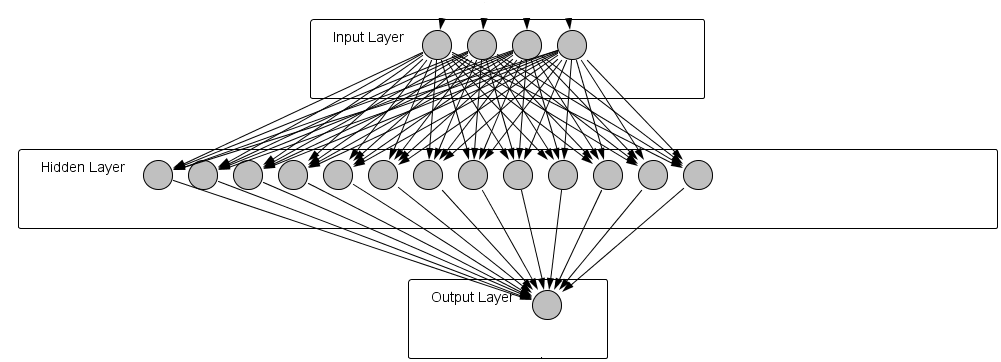
\includegraphics[width=0.75\textwidth]{4-13-1.PNG}
	\caption{KNN nach 4-13-1 Muster}
	\label{fig:KNN nach 4-13-1 Muster}
\end{figure}


\begin{table}
  \centering
  \begin{tabular}{|c|c|}
  \hline 
  \rule[0ex]{0pt}{2.5ex} Topologie & Mean Squared Error \\ 
  \hline 
  \rule[0ex]{0pt}{2.5ex} 4-05-1 & 0.000 \\ 
  \hline 
  \rule[0ex]{0pt}{2.5ex} 4-09-1 & 0.000 \\ 
  \hline 
  \rule[0ex]{0pt}{2.5ex} 4-13-1 & 0.000 \\ 
  \hline 
  \end{tabular} 
  \caption{Jeweilige Topologien \& korrespondierende MSE}
  \label{tab:myfirsttable}
\end{table}


\subsection{Wahl der optimalen Transferfunktion} %Sebastian

Sigmoide Funktion:

\begin{equation}\formelentry{Sigmoide Funktion}
f(x)= \frac{1}{1+e^{-cx}}
\end{equation}

\begin{figure}[htbp]
\centering
		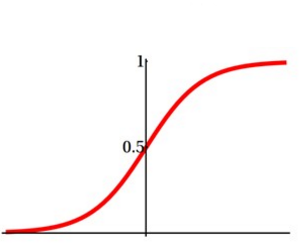
\includegraphics[width=0.5\textwidth]{Sigmoid.PNG}
	\caption{Sigmoide Funktion}
	\label{fig:Sigmoide Funktion}
\end{figure}

Tangens Hyperbolicus:

\begin{equation}\formelentry{Tanh Funktion}
f(x)= tanh(x)
\end{equation}

\begin{figure}[htbp]
\centering
		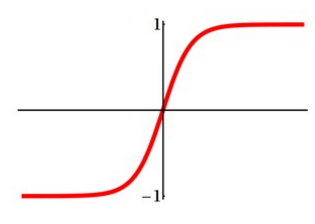
\includegraphics[width=0.5\textwidth]{tanh.PNG}
	\caption{Tangens Hyperbolicus Funktion}
	\label{fig:Tangens Hyperbolicus Funktion}
\end{figure}

\begin{table}
  \centering
  \begin{tabular}{|c|c|}
  \hline 
  \rule[0ex]{0pt}{2.5ex} Transferfunktion & Mean Squared Error \\ 
  \hline 
  \rule[0ex]{0pt}{2.5ex} 4-05-1 & 0.000 \\ 
  \hline 
  \rule[0ex]{0pt}{2.5ex} 4-09-1 & 0.000 \\ 
  \hline 
  \rule[0ex]{0pt}{2.5ex} 4-13-1 & 0.000 \\ 
  \hline 
  \end{tabular} 
  \caption{Jeweilige Transferfunktionen \& korrespondierende MSE}
  \label{tab:tab2}
\end{table}

\subsection{Wahl der optimalen Lernregel} %Sebastian

\begin{table}[H]
  \centering
  \begin{tabular}{|c|c|c|}
  \hline 
  \rule[0ex]{0pt}{2.5ex} Lernregel & beste Lernrate & Mean Squared Error \\ 
  \hline 
  \rule[0ex]{0pt}{2.5ex} Backpropagation & 0.000 & 0.000 \\ 
  \hline 
  \rule[0ex]{0pt}{2.5ex} Momentum Backpropagation & 0.000 & 0.000\\ 
  \hline 
  \rule[0ex]{0pt}{2.5ex} Resilient Propagation & 0.000 & 0.000 \\ 
  \hline 
  \end{tabular} 
  \caption{Jeweilige Lernregeln und beste Lernraten \& korrespondierende MSE}
  \label{tab:tab3}
\end{table}
\section{Das erstellte künstliche neuronale Netz}

\section{Zusammenführung der Komponenten}
